\chapter{实数}
\section{集合与映射}
\precis{集合,关系与映射,Descartes 乘积,函数,集合的势,可数集,不可数集,代数数,超越数,Bernstein定理}
\begin{tcolorbox}
列入\(\mathcal{A} \)的习题相对基础, 列入\(\mathcal{B}\)的习题相对困难或属于扩展问题, 个别习题可能超前. 若习题中加*号, 表示该习题与后续内容相关性大, 请教师布置习题时, 尽量勾选该题.
\end{tcolorbox}
\begin{theorem}{关于Diophantus逼近的Liouville定理}{C11}
    设\(n\geqslant 2\), 无理数\(x\)是某个\(n\)次整系数多项式的零点, 则存在常数\(A\)使得对于任何整数\(q\)和正整数\(p\),成立\[\left|x-\frac{q}{p}\right|>\frac{A}{p^n}.\]
\end{theorem}
\begin{quiza}
\woe 设\(a_0,a_1,\cdots,a_n\)为复常数, 且对任何\(x\in \mathbb{R}\) 成立 \[a_nx^n+a_{n-1}x^{n-1}+\cdots+a_1x+a_0=0.\]证明:\(a_0=a_1=\cdots=a_n=0\).
\begin{proof}
令\(x_0=0\)代入\(x\)可得\(a_0=0\). 分别令\(x=x_i,(i=1,2,\cdots,n)\)满足\(x_i\ne x_j\)\(j=0,1,\cdots,n\). 可得如下关于\(a_1,a_2,\cdots,a_n\)的方程组.
        \[\begin{cases}
            a_1x_1+a_2x_1^2+\cdots+a_nx^n_1=0\\
            a_1x_2+a_2x_2^2+\cdots+a_nx^n_2=0\\
            \cdots\\
            a_1x_n+a_2x_n^2+\cdots+a_nx^n_n=0\\
        \end{cases}\]
        其系数矩阵的行列式为
        \[\left|\begin{matrix}
            x_1&x_1^2&\cdots&x_1^n\\
            x_2&x_2^2&\cdots&x_2^n\\
            \vdots&\vdots&&\vdots\\
            x_n&x_n^2&\cdots&x_n^n\\
        \end{matrix}\right|=\prod_{i=1}^{n}x_i\left|\begin{matrix}
            1&x_1&x_1^2&\cdots&x_1^{n-1}\\
            1&x_2&x_2^2&\cdots&x_2^{n-1}\\
            \vdots&\vdots&\vdots&&\vdots\\
            1&x_n&x_n^2&\cdots&x_n^{n-1}\\
        \end{matrix}\right|=\prod_{i=1}^{n}x_i\prod_{1\leqslant i<j\leqslant n}^{n}(x_i-x_j)\ne 0.\]
        故原方程仅有零解, 这便证明了结论. \hfill\qedsymbol
        \tcbline
        
        或者令\(x=0\), 立即得\(a_0=0\), 于是得到\[a_nx^n+a_{n-1}x^{n-1}+\cdots+a_1x=0.\]上式两端除以\(x\), 此时假定\(x\ne 0\), 得到\[a_nx^{n-1}+a_{n-1}x^{n-2}+\cdots+a_1=0,\]令\(x=0\)得到\(a_1=0\). 循环该流程, 可得结论.
\end{proof}
\woe 试构造区间\(\left(0,1\right)\)到\(\left[0,1\right]\)的一个双射。
\begin{solution}
设集合
    \[T=\left\lbrace\frac{1}{2},\frac{1}{2^2},\cdots,\frac{1}{2^n},\cdots\right\rbrace,\]构造如下映射\[f(x)=\begin{cases}
        x,\qquad &x\notin T,\\
        0, &x=\frac{1}{2},\\
        4x,& x\in T,x\ne \frac{1}{2}.
    \end{cases}\]
    可以观察出, 这是一个符合题目要求的双射. 另外还可以分别拿出这两个集合的有理数, 对于集合\([0,1]\), 其所有有理数组成集合为\[\left\lbrace a_0,a_1,a_2,\cdots,a_n,\cdots \right\rbrace,\] 这里规定\(a_0=0,a_1=1.\)对于集合\((0,1)\), 类似有\[\left\lbrace a_2,\cdots,a_n,\cdots \right\rbrace,\] 定义映射如下\[f(x)=\begin{cases}
        x,\qquad &x\in \mathbb{R}\backslash\mathbb{Q},\\
        a_{n-2}&x=a_n.
    \end{cases}\hfill\qedhere\]
\end{solution}
\woe 说明以下映射为有理数到整数集的单射.\[T(q)=\begin{cases}
        (m+n)^2+n,\qquad & q=\frac{n}{m},m,n \text{为既约正整数},\\
        0,&q=0,\\
        -(m+n)^2-n,\qquad & q=-\frac{n}{m},m,n \text{为既约正整数}.
    \end{cases}\]
\begin{proof}
不妨设\(q_1=n_1/m_1,q_2=n_2/m_2\),\(m,n\)为既约正整数且\(q_1\ne q_2.\) 若\(n_1=n_2\)且\(m_1\ne m_2\)或\(m_1=m_2\)且\(n_1\ne n_2\), 显然有\(T(q_1)\ne T(q_2)\). 

下证\(n_1\ne n_2\,,m_1\ne m_2\)的情形. 不失一般性, 我们设\(n_1>n_2\). 此时, 若\(T(q_1)=T(q_2)\)即\[(m_1+n_1)^2+n_1=(m_2+n_2)^2+n_2\]必有\(m_1+n_1<m_2+n_2\). 设\(t=m_1+n_1\), 得到\[m_2+n_2=t+[(m_2+n_2)-(m_1+n_1)]:=t+k.\]
显然\(k>1,t>n_1\), 于是\[\begin{split}
    (m_2+n_2)^2-(m_1+n_1)^2-n_1&=(t+k)^2-t^2-n_1\\
    &=k^2+2kt-n_1>0.
\end{split}\]
即若\((m_2+n_2)^2>(m_1+n_1)^2\)必有\[(m_2+n_2)^2>(m_1+n_1)^2+n_1\]可见此时不可能有\(T(q_1)=T(q_2)\). \(q<0\)的情况可类似说明.
\end{proof}
\woe 证明代数数集是可列集.
\begin{proof}
设\(P_n(x)\)为\(n\)次整系数多项式构成的集合. \(U_n\)为所有\(n\)次整系数多项式的复零点, 由于对于一个确定的\(n\)次多项式\[f(x)=a_0+a_1x+a_2x^2+\cdots+a_nx^n\]它的零点为有限多个. 由于可列个可列集的并为可列集, 接下来我们证明\(P_n(x)\)为可列集. 记\(p(n)\)为第\(n+1\)个素数.

定义如下映射\[f(x)\mapsto\prod_{j=0}^{n}\left(p(j)\right)^{a_j}.\]
这便建立了一个\(P_n(x)\)到\(\mathbb{N}\)的一个双射, 从而\(P_n(x)\)为可列集, 故其元素的复零点的并集为\(U_n\)也为可列集, 从而代数数集\(\underset{n}{\bigcup}\,U_n\)为可列集.
\end{proof}
\woe 证明:存在常数\(A>0\)使得对于任何整数\(q\)和正整数\(p\)成立\[\left|\sqrt{3}-\frac{q}{p}\right|>\frac{A}{p^2}\]
\begin{proof}
\(\sqrt{3}\)为\(x^2-3\)的一个零点, 根据定理\ref{Th:C11}可知结论成立.
\end{proof}
\end{quiza}
\begin{quizb}
\woe 设\(P\)为首项系数不为零的\(n\)次系数多项式, \(x_1\)是它的一个零点, 则存在首项系数不为零的\(n-1\)次多项式\(Q\)使得\[P(x)=(x-x_1)Q(x).\]
\begin{proof}
由于\[x^k-x_1^k=(x-x_1)\left(x^{k-1}+x_1x^{k-2}+\cdots+x_1^{k-2}x+x_1^{k-1}\right).\]则对\(P(x)\)中的每项应用上述事实便得到了结论.
\end{proof}
\woe 设\(a_0,a_1,\cdots,a_n\)为复常数, \(a_n\ne 0\).证明:多项式\[P(x)=a_nx^n+a_{n-1}x^{n-1}+\cdots+a_1x+a_0\]至多有\(n\)个复零点(含重数).
\begin{proof}
这正是代数基本定理, 这个定理的第一个严格证明是1799年由Gauss证明的, 后来他又给出了4个证明, Jordan, Weyl等人也给过这个定理的证明. 它的一般表述是: 次数大于零的复数域上的多项式至少有一复数根.
\end{proof}
\woe 证明 Vi\`{e}te (韦达) 定理:设\(a_n\ne 0,x_1,x_2,\cdots,x_n\)为\[P(x)=a_nx^n+a_{n-1}x^{n-1}+\cdots+a_1x+a_0\]的\(n\)个复零点(含重根), 则对于\(1\leqslant k\leqslant n\), 成立 \[\sum_{1\leqslant m_1<m_2<\cdots<m_k\leqslant n}\,\prod_{j=1}^{k}x_{m_j}=(-1)^k \frac{a_{n-k}}{a_n}.\]
\begin{proof}
由前面的两个问题可以知道\[P(x)=a_n(x-x_1)(x-x_2)\cdots(x-x_n).\]即有\[(x-x_1)(x-x_2)\cdots(x-x_n)=x^n+\frac{a_{n-1}}{a_n}x^{n-1}+\cdots+\frac{a_1}{a_n}x+\frac{a_0}{a_n}\]比较系数便得到了结果.
\end{proof}
\woe 称关于\(x_1,x_2,\cdots,x_n\)的\(m\)次\(n\)元多项式\(R(x_1,x_2,\cdots,x_n)\)是\textbf{可轮换的}, 如果对任何\(1\leqslant k<j\leqslant n\), 将\(R(x_1,x_2,\cdots,x_n)\)中的\(x_k,x_j\)分别替换成\(x_j,x_k\)后多项式的值保持不变. 证明: 
\begin{quizs}
\item 若\(R(x_1,x_2,\cdots,x_n)\)是可轮换的一次多项式, 则它是\(x_1+x_2+\cdots+x_n\)的常数倍.
\item 若\(R(x_1,x_2,\cdots,x_n)\)是可轮换的二次多项式, 则有常数\(C_1,C_2\)使得\[R(x_1,x_2,\cdots,x_n)=C_1(x_1^2+x_2^2+\cdots+x_n^2)+C_2\sum_{1\leqslant i<j\leqslant n }x_ix_j.\]
\item 归纳证明, 若\(R(x_1,x_2,\cdots,x_n)\)是\textcolor{green!50!black}{系数为有理数的}可轮换的\(k\)次多项式, 而\(x_1,x_2,\cdots,x_n\)是某首项系数不为零的\(n\)次有理系数多项式的零点, 则\(R(x_1,x_2,\cdots,x_n)\)为有理数.
\end{quizs}
\begin{proof}
(1)(2)是容易证明的, 下面我们证明(3).
这证明这个结论之前, 我们先引入几个有用的记号(称为\(n\)元初等对称多项式):\[\begin{split}
\sigma_1&=x_1+x_2+\cdots+x_n=\sum_{n=1}^{n}x_i,\\
\sigma_2&=x_1x_2+x_1x_3+\cdots+x_{n-1}x_n=\sum_{1\leq i<j\leq n }x_ix_j,\\
&\qquad\qquad\qquad\cdots\cdots\cdots\cdots\\
\sigma_n&=x_1x_2\cdots x_n.
\end{split}\]
事实上我们有如下定理, 称为\textbf{对称多项式基本定理}: 设\(f(x_1,x_2,\cdots,x_n)\)是数域\(\mathbb{K}\)上的对称多项式, 则必存在\(\mathbb{K}\)上唯一的一个多项式\(g(y_1,y_2,\cdots,y_n)\), 使\[f(x_1,x_2,\cdots,x_n)=g(\sigma_1,\sigma_2,\cdots,\sigma_n).\]
对称多项式的定义如同可轮换, 但不要求齐次性, 所以\(m\)次的可轮换多项式为对称多项式. 如果我们证明了定理中\(g\)的存在性, 那么根据Vi\`{e}te定理, 则本题即证. 下面用归纳法证明存在性, 唯一性参考相关书籍.

我们对\(n\)与多项式\(f\)的次数\(\deg f\)进行归纳. 当\(n=1\)或\(\deg f=0\)或\(1\), 结论显然成立, 假设结论对于\(n-1\)与小于给定次数\(\deg f\)的对称多项式成立. 考虑\[g(x_1,x_2,\cdots,x_{n-1})=f(x_1,x_2,\cdots,x_{n-1},0),\]我们以\(\sigma'_1,\sigma'_2,\cdots,\sigma'_{n-1}\)表示\(x_1,x_2,\cdots,x_{n-1}\)的基本初等对称多项式, 由归纳假设知有\(h(y_1,y_2,\cdots,y_{n-1})\)使得\[g(x_1,x_2,\cdots,x_{n-1})=h(\sigma'_1,\sigma'_2,\cdots,\sigma'_{n-1}),\]若\(h=0\), 则\(x_n\big| f\), 又由于\(f\)为对称多项式, 则\(x_1x_2\cdots x_n\big| f\), 考虑对称多项式\(\frac{f}{x_1x_2\cdots x_n}\), 它的次数为\(\deg f -n\). 

若\(h\ne 0\), 考虑\[h'=f(x_1,x_2,\cdots,x_{n})-h(\sigma_1,\sigma_2,\cdots,\sigma_{n-1}),\]
易见\(x_n=0\)时\(h'=0\), 类似\(h=0\)的讨论考虑\(\frac{h'}{x_1x_2\cdots x_n}\), 它的次数也为\(\deg f -n\). 依归纳假设便完成了证明.
\end{proof}
\woe 设\(P,Q\)分别是\(m,n\)阶首项系数为1的有理系数多项式.\[P(x)=\prod_{k=1}^{m}(x-x_k),\quad Q(x)=\prod_{k=1}^{n}(x-y_k).\]证明:
        \begin{quizs}
            \item 多项式\(R(x)=\prod_{k=1}^{m}\prod_{j=1}^{n}(x-x_k-y_j)\)是有理系数多项式.
            \item 多项式\(S(x)=\prod_{k=1}^{m}\prod_{j=1}^{n}(x-x_ky_j)\)是有理系数多项式.
        \end{quizs}
\woe 证明Liouville定理, 即定理\reff{Th:C11}.
\begin{proof}
设无理数\(x_0\)是整系数多项式\[f(x)=a_nx^n+a_{n-1}x^{n-1}+\cdots+a_1x+a_0\]的零点, 令\(M=\max_{x_0-1<x<x_0+1}\{|f'(x)|\}\), \(f(x)\)其他互异的零点为\(x_1,x_2,\cdots,x_m\). 取\(A\)满足\(0<A<\min\left\lbrace 1,\frac{1}{M},|x_0-x_1|,|x_0-x_2|,\cdots,|x-x_m| \right\rbrace\). 假设存在使定理不成立的\(p,q\), 就有\[\left|x_0-\frac{q}{p}\right|\leqslant\frac{A}{p^n}\leqslant A<\min\left\lbrace 1,\frac{1}{M},|x_0-x_1|,|x_0-x_2|,\cdots,|x-x_m| \right\rbrace\leqslant 1,\]那么有
\begin{gather*}
x_0-1<\frac{q}{p}<x_0+1,\text{并且}\,\frac{q}{p}\notin\{x_1,x_2,\cdots,x_m\},\\
\left|f\left(\frac{q}{p}\right)\right|=\frac{\left|a_nq^n+a_{n-1}q^{n-1}p+\cdots+a_1qp^{n-1}+a_0p^n\right|}{p^n}\geqslant\frac{1}{p^n}.
\end{gather*}根据Lagrange中值定理, 存在\(\xi\)位于\(\frac{q}{p}\)与\(x_0\)之间, 使得\(\frac{f}{x_0}-f\left(\frac{q}{p}\right)=f'(\xi)\left(x_0-\frac{q}{p}\right)\), 又根据\(M,K\)的定义, 得到\[\left|x_0-\frac{q}{p}\right|=\frac{|f(x_0)-f(q/p)|}{|f'(\xi)|}\geqslant\frac{1}{MP^n}>\frac{K}{p^n}\geqslant\left|x_0-\frac{q}{p}\right| ,\]矛盾, 从而结论得证.
\end{proof}
\woe 证明一个复数是代数数当且仅当它的实部和虚部都是代数数.
\end{quizb}
\section{第一次数学危机}
\precis{第一次数学危机,可公度量,比例论}
\begin{quiza}

\woe  在有关讲座中, 项武义教授给出了图 \ref{c1t1}. 从中可见, 当\(a,b\)依次是正五边形的边长和对角线长时, \(b-a\)和\(a\)时一个更小的正五边形的边长和对角线. 试以此说明正五边形的边长和对角线长不可公度.
 \begin{figure}[H]
    \centering
    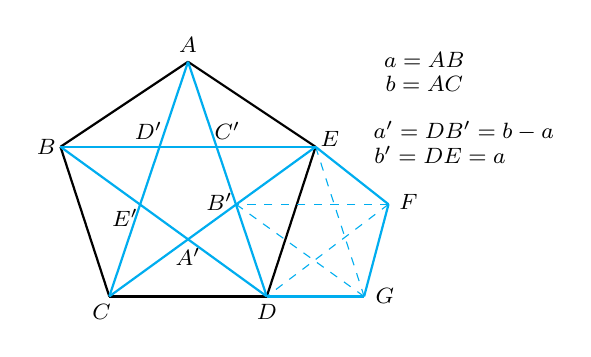
\begin{tikzpicture}
     \draw[thick]  (0,0)--(2,0);\draw[thick]  (2,0)--(2.62,1.90);\draw[thick]  (2.62,1.90)--(1,2.98);
     \draw[thick] (1,2.98)--(-0.62,1.90);\draw[thick] (0,0)--(-0.62,1.90);
      \draw[thick,color=cyan] (0,0)--(2.62,1.90);\draw[thick,color=cyan] (2.62,1.90)--(-0.62,1.90);
                \draw[thick,color=cyan] (1,2.98)--(0,0);\draw[thick,color=cyan] (2,0)--(-0.62,1.90);
                \draw[thick,color=cyan] (2,0)--(1,2.98); 
                \draw[thick,color=cyan] (2,0)--(3.236,0);\draw[thick,color=cyan] (3.236,0)--(3.546,1.17);
                \draw[thick,color=cyan](3.546,1.17)--(2.62,1.90);\draw[dashed,color=cyan](2.62,1.90)--(3.236,0);
                \draw[dashed,color=cyan](3.546,1.17)--(2,0);\draw[dashed,color=cyan](3.546,1.17)--(1.61,1.17);
                \draw[dashed,color=cyan](1.61,1.17)--(3.236,0);
                \node at (-0.8,1.9) {\footnotesize $B$};\node at (-0.1,-0.2) {\footnotesize$C$};
                \node at (2,-0.2) {\footnotesize$D$};\node at (1,3.2) {\footnotesize$A$};
                \node at (2.8,2) {\footnotesize$E$};\node at (3.8,1.2) {\footnotesize$F$};
                \node at (3.5,0) {\footnotesize$G$};\node at (0.5,2.1) {\footnotesize$D'$};
                \node at (1.5,2.1) {\footnotesize$C'$};\node at (0.2,1) {\footnotesize$E'$};
                \node at (1.,0.5) {\footnotesize$A'$};\node at (1.4,1.2) {\footnotesize$B'$};
                \node at (4,3) {\footnotesize $a=AB$};\node at (4,2.7) {\footnotesize $b=AC$};
                \node at (4.5,2.1) {\footnotesize $a'=DB'=b-a$};\node at (4.2,1.8) {\footnotesize $b'=DE=a$};
            \end{tikzpicture}
 \caption{}
\label{c1t1}
\end{figure}
\tcbline
若正五边形的边和对角线可公度, 则可以把\(a,b\)视为正整数, 此时\(a',b'\)也是正整数, 且\(a'<a,b'<b\). 易见小于\(a\)的正整数只有有限个, 因此这一过程不可能无限持续, 这表明正五边形的边和的对角线不可公度.
\tcbline
\woe 结合图 \ref{c1t2} 说明等腰直角三角形直角边和斜边长不可公度.
        \begin{figure}[H]
            \centering
            \begin{tikzpicture}
                \draw[thick,color=cyan](0,0)--(3,0);\draw[thick,color=cyan](3,3)--(3,0);
                \draw[thick,color=cyan](0,0)--(0,3);\draw[thick,color=cyan](3,3)--(0,3);
                \draw[thick,color=cyan](0,2)--(2,2);\draw[thick,color=cyan](2,0)--(2,2);
                \draw[thick,color=cyan](3,1)--(1,1);\draw[thick,color=cyan](1,3)--(1,1);
                \draw[-](-0.3,0)--(-0.1,0);\draw[-](-0.3,3)--(-0.1,3);
                \draw[-latex](-0.2,1.65)--(-0.2,3);
                \draw[-latex](-0.2,1.35)--(-0.2,0);
                \node at (-0.2,1.5) {$c$};
                \draw[-latex](0.2,1.15)--(0.2,2);
                \draw[-latex](0.2,0.85)--(0.2,0);
                \node at (0.2,1) {$a$};\node at (1,0.2) {$a$};
                \node at (2.8,2) {$a$};
                \node at (4.5,2.8){\footnotesize 若$c^2=2a^2$};
                \node at (5.3,2.4){\footnotesize 则$(2a-c)^2=2(c-a)^2$};
            \end{tikzpicture}
            \caption{}
            \label{c1t2}
        \end{figure}
\tcbline
若\(c^2=2a^2\), 依勾股定理, \(c\)是直角边为\(a\)的等腰直角三角形的斜边. 依图可令\(c'=2a-c,a'=c-a\), 若\(c,a\)可公度, 则可视为正整数,此时\(a',c'\)也是正整数, 且\(c'<c\), 但小于\(c\)的正整数有限, 这一流程不可能无限持续, 因而等腰直角三角形直角边和斜边不可公度.
\end{quiza}
\begin{quizb}
\woe 对于正整数\(n,m\), 考察\(\frac{m}{n}\)的十进制小数表示中循环节的长度有何特点.
\tcbline
只考虑\(n>m\)的情况, 当\(n=9,99,999,\cdots\)时, 分数的结果都是循环小数, 且循环节的长度与\(n\)的位数相同.对于一个给定的循环小数\(a=0.a_1a_2\cdots a_na_1a_2\cdots\), (\(a_i\)表示当前位数上的数字), 有\begin{gather*}
            10^na-a=a_1a_2\cdots a_n\\
            a=\frac{a_1a_2\cdots a_n}{10^n-1}
            \end{gather*}
\end{quizb}
\section{实数公理系统}
\precis{自然数公理,数学归纳法,实数公理系统,实数系,有序域的性质,三角不等式,Newton二项展开式,杨辉三角,广义实数系,区间,单调函数,复数域,周期函数}
\begin{quiza}
\woe 设\((X,+,\cdot,\leqslant)\)是一个有序域, 并用\(0^*,1^*\)表示\(X\)的零元和单位元. 一般的, \(n^*=n1^*\). 我们可以证明\(X\)中成立\textbf{加法消去律}: 设\(\alpha,\beta,\gamma\in X\), 满足条件\(P:\alpha+\gamma=\beta+\gamma\), 则
\[\begin{split}
\alpha&\ndtstile{{}}{{(A3)}}\alpha+0^*\ndtstile{{}}{{(A4)}}\alpha+\left(\gamma+(-\gamma)\right)\ndtstile{{}}{{(A1)}}(\alpha+\gamma)+(-\gamma)\\
&\ndtstile{{}}{{P}}(\beta+\gamma)+(-\gamma)\ndtstile{{}}{{(A1)}}\beta+\left(\gamma+(-\gamma)\right)=\beta+0^*=\beta.
\end{split}\]类似的证明: 
\begin{quizcs}
\item 若\(\alpha\geqslant \beta\), 则\(\alpha+\gamma\geqslant \beta+\gamma\), 且等号当且仅当\(\alpha=\beta\)时取到.
\item \(\alpha>0^*\)当且仅当\(-\alpha<0^*\).
\item 若\(\alpha\gamma=\beta\gamma\), 且\(\gamma\ne 0^*\), 则\(\alpha=\beta\).
\item \(\alpha^2\geqslant 0^*\), 且等号成立当且仅当\(\alpha=0^*\)时成立. 特别的\(1^*>0^*\).
\item \(\alpha>0^*\)当且仅当\(1/\alpha>0^*\).
\item 设\(\alpha>0,\beta>\gamma\), 则\(\alpha\beta>\alpha\gamma.\)
\end{quizcs}
\begin{proof}
(1) 若\(\alpha>\beta\)有\(\alpha+\gamma=\beta+\gamma\), 依\textbf{加法消去律}可知有\(\alpha=\beta\), 与假设矛盾. 反之若\(\alpha=\beta\), 依上述也有\(\alpha+\gamma=\beta+\gamma\).

(2) \(\alpha>0^*=\alpha+(-\alpha)\), 依消去律得\(-\alpha<0^*\).

(3)\(\alpha=\alpha 1^*=\alpha(\gamma\gamma^{-1})=(\alpha\gamma)\gamma^{-1}=\beta\gamma\gamma^{-1}=\beta.\)

(4)先证 \((-1^*)(-1^*)=1^*\):\[\begin{split}
                1^*+(-1^*)=0^*&\Rightarrow (-1^*)*(1^*+(-1)^*)=0^*\Rightarrow -1^*+(-1^*)(-1^*)=0^*\\
                &\Rightarrow (-1^*)(-1^*)=1^*.
            \end{split}\]
若\(\alpha\geqslant 0\), 依乘法的保序性可知\(\alpha^2\geqslant 0\), 并且若\(\alpha>0\)而\(\alpha^2=0^*\), 则两侧乘以\(\alpha^{-1}\)得\(\alpha=0^*\), 可得矛盾. 从而若\(\alpha^2=0^*\)必有\(\alpha= 0^*\).若\(\alpha <0^*\), 则\(-\alpha>0^*\),从而\[\alpha\alpha=1^*\cdot \alpha\cdot\alpha=(-1^*)(-1^*)\alpha\alpha=(-\alpha)(-\alpha)>0^*.\]

(5)设\(\alpha>0,\beta<0\), 则\(-\beta>0\), 从而\(\alpha(-\beta)>0^*\), 于是\(\alpha\beta<0\).若\(\alpha>0\)而\(1/\alpha<0\), 则\[\alpha\cdot 1/\alpha=1^*<0^*\]矛盾.

(6)由于\(\alpha>0,\beta-\gamma>0\), 从而\(\alpha(\beta-\gamma)>0\). 可得\(\alpha\gamma>\alpha\gamma.\)
\end{proof}
\woe 设\((X,+,\cdot,\leqslant)\)是一个全序域, \(\alpha\in X\)满足\(\alpha\geqslant 0\)以及\(\forall \varepsilon>0\), 成立\(\alpha<\varepsilon\). 证明\(\alpha=0.\)
\begin{proof}
假设\(\alpha>0\), 则令\(\varepsilon=\alpha\), 则与\(\alpha<\varepsilon\)矛盾. 从而\(\alpha=0\).
\end{proof}
\end{quiza}
\begin{quizb}
\woe 对于有序域\((X,+,\cdot,\leqslant)\), 是否一定具有Archimedes性?
\woe 设\((X,+,\cdot,\leqslant)\)是一个全序域, \(\alpha\in X\)满足\(\alpha\geqslant 0\)以及对\(X\)中任何的正有理数\(p\)成立\(\alpha<p\). 问是否一定有\(\alpha=0\)?\\ 这里正有理数即形如\(m1^*/n1^*\)的元, 其中\(1^*\)为乘法单位元, \(m,n\)为正整数.
\woe 证明所有(复)代数数组成的集合是一个域.
\begin{proof}
内容...
\end{proof}
\woe 设\((X,+,\cdot)\)是一个以实数域\(\mathbb{R}\)为子域的域, 满足如下条件:\begin{compactenum}[(i)]
\item 存在元\(A\in X\backslash\mathbb{R}\).
\item 对于\(X\)中的任一元素\(V\), 都存在\(a,b\in \mathbb{R}\), 使得\(V=a+bA\).
\end{compactenum}
证明:存在\(B\in X\)使得\(B^2=-1\). 进一步, 对\(X\)中的任一元素\(V\), 都存在\(a,b\in \mathbb{R}\), 使得\(V=a+bB\).\\本题的结论相当于说, 以实数域作为子域的“二元域”一定是复数域.
\woe 证明: 不存在以\(\mathbb{R}\)为子域的“三元数”域. 即不存在\(\mathbb{R}^3\)中满足\[(x_1,y_1,z_1)+(x_2,y_2,z_2)=(x_1+x_2,y_1+y_2,z_1+z_2)\]以及\[(x_1,0,0)\cdot (x_2,0,0)=(x_1x_2,0,0)\]的加法\(+\)和乘法\(\cdot\), 使得\((\mathbb{R}^3,+,\cdot)\)成为一个域.
\end{quizb}
\section{实数系的构造}
\precis{实数系的构造,Dedekind分割,稠密性,上确界存在定理,有理数,无理数,实数的十进制表示,\(n\)次方根,算术几何平均不等式,指数函数的定义,对数函数的定义}
\begin{quiza}
\woe  Rudin 在其《数学分析原理》一书中使用了变换\(q=p+\frac{2-p^2}{p+2}=\frac{2+2p}{p+2}\). 验证:
\begin{compactenum}[(i)]
            \item 若\(p>0\), 且\(p^2<2\), 则\(q>p\)且\(q^2<2\).
            \item 若\(p>0\), 且\(p^2>2\), 则\(0<q<p\)且\(q^2>2\).
\end{compactenum}
\begin{solution}
由\(p>0\)且\(p^2<2\)易知\(q=p+\frac{2-p^2}{p+2}>p\), 并且\[q^2=\left(\frac{2+2p}{p+2}\right)^2=4\left(1-\frac{1}{p+2}\right)^2<4\left(1-\frac{1}{\sqrt{2}+2}\right)^2=2.\]后者情况类似.
\end{solution}
\woe 试求使变换\(q=p+\frac{2-p^2}{ap+b}\)具有习题\textbf{1}中性质(i)---(ii)的所有有理数对\((a,b)\).
\begin{solution}

\end{solution}
\woe 证明无理数在实数集中的稠密性: 对于任何\(x\in \mathbb{R}\), 以及\(\varepsilon>0\), 存在无理数\(y\)使得\(|y-x|<\varepsilon\).
\begin{proof}
内容...
\end{proof}
\woe 设\(a>0\), 而\(n\)为正整数. 证明: \(\min \{a,1\}\leqslant a^{1/n}\leqslant\max\{a,1\}\).
\begin{proof}
易见\(a\in (0,1)\)时, 有\(a\leqslant a^{1/n}\leqslant 1\); 若\(a\geqslant1\), 则\(1\leqslant a^{1/n}<a\). 总而言之有 \(\min \{a,1\}\leqslant a^{1/n}\leqslant\max\{a,1\}\).
\end{proof}
\woe 设\(p,q>1\)满足\(\frac{1}{p}+\frac{1}{q}=1,a,b>0\). 利用
\begin{equation}\label{c1e1}\tag{\(\heartsuit\)}
(1+x)^\alpha-1\leqslant \alpha x,\qquad x\geqslant 0,0<\alpha\leqslant1
\end{equation}
证明Young不等式: \(ab\leqslant\frac{1}{p}a^p+\frac{1}{q}b^q\).
\begin{proof}
不妨设\(a^p>b^q\), 则令\(x=\frac{a^p}{b^q}-1,\alpha=\frac{1}{p}\)带入式\eqref{c1e1}得到\[\frac{a}{b^{q/p}}-1\leqslant \frac{1}{p}\left(\frac{a^p}{b^q}-1\right),\]即\(ab\leqslant\frac{1}{p}a^p+\frac{1}{q}b^q\). 另外的情况类似.
\end{proof}
\woestar 设\(I\)是一个非空指标集, 对\(I\)中每一个元\(\alpha\), 都对应两个实数\(x_\alpha\)以及\(y_\alpha\). 我们将\(\sup\{x_\alpha|\alpha\in I\}\)和\(\inf\{x_\alpha|\alpha\in I\}\)写成\(\underset{\alpha\in I}{\sup}\,x_\alpha\)和\(\underset{\alpha\in I}{\inf}\,x_\alpha\). 证明: 在广义实数系中,
\begin{quizs}
 \item \(\underset{\alpha\in I}{\inf}(-x_\alpha)=-\underset{\alpha\in I}{\sup}\,x_\alpha\).
\item 对以下所列的每一个不等式, 若其两端在广义实数系中都有意义, 则该不等式成立:\[\begin{split}
\underset{\alpha\in I}{\inf}\,x_\alpha+\underset{\alpha\in I}{\inf}\,y_\alpha&\leqslant\underset{\alpha\in I}{\inf}(x_\alpha+y_\alpha)\leqslant\underset{\alpha\in I}{\sup}\,x_\alpha+\underset{\alpha\in I}{\inf}\,y_\alpha\\&\leqslant\underset{\alpha\in I}{\sup}(x_\alpha+y_\alpha)\leqslant\underset{\alpha\in I}{\sup}\,x_\alpha+\underset{\alpha\in I}{\sup}\,y_\alpha.\end{split}\]
\item 若\(x_\alpha>0(\forall \alpha\in I)\), 并在此种情形规定\(\frac{1}{0}=+\infty\), 则有\[ \underset{\alpha\in I}{\sup}\,\frac{1}{x_\alpha}=\frac{1}{\underset{\alpha\in I}{\inf}\,x_\alpha}.\]
\item 设\(x_\alpha>0,y_\alpha>0\,(\forall \alpha\in I)\). 对以下所列的每一个不等式, 若其两端在广义实数系中都有意义, 则该不等式成立: \[\begin{split}
\underset{\alpha\in I}{\inf}\,x_\alpha\underset{\alpha\in I}{\inf}\,y_\alpha&\leqslant \underset{\alpha\in I}{\inf}(x_\alpha y_\alpha)\leqslant\underset{\alpha\in I}{\sup}\,x_\alpha\underset{\alpha\in I}{\inf}\,y_\alpha\\&\leqslant
\underset{\alpha\in I}{\sup}(x_\alpha y_\alpha)\leqslant\underset{\alpha\in I}{\sup}\,x_\alpha\,\underset{\alpha\in I}{\sup}\,y_\alpha.
\end{split}\]
\end{quizs}
\begin{proof}
(1)

(2)

(3)

(4)
\end{proof}
\end{quiza}
\begin{quizb}
\woe 对于\(a>0\)以及有理数\(\frac{m}{n}\), 其中\(m,n\)为既约整数, \(n>0\). 当\(m\ne 1\)时, 定义\[a^{\frac{m}{n}}=\left(a^m\right)^\frac{1}{n}\]
        自然, 当\(m=1\)时, 上式也成立. 进一步, 当\(n=2k+1\)为奇数时, 定义\[(-a)^{m/(2k+1)}=(-1)^ma^{m/2k+1}.\]下设\(a,b>0\), 且\(p,q\)为有理数, 证明:
\begin{compactenum}[\quad (1)]
            \item \((a^p)^q=a^{pq}\).
            \item \(a^pa^q=a^{p+q}\).
            \item \(a^pb^p=(ab)^p\).
            \item 若\(a>1,p>0\), 则\(a^p>1\).
            \item 当\(a>1\)时, \(a^p\)关于\(p\in\mathbb{Q}\)严格单调递增.
            \item 设\(a>1\), 证明: 对于任何\(b\in\mathbb{R}\), 成立\(\mathrm{sup}\{a^p|p<b\}=\mathrm{inf}\{a^p|p>b.\}\)
\end{compactenum}
\woe 设\(a\geqslant 1\), 且\(b\)为无理数, 定义\[a^b=\sup\{a^p|p\leqslant b \text{ 且 }p\text{ 为有理数}\}.\]
证明: 当\(p\)为有理数时上式也成立. 

进一步, 当\(0<a<1\)时, 定义\(a^b=(a^{-1})^{-b}\).
\woe 设\(a,b>0\), 且\(x,y\in \mathbb{R}\), 证明:
\begin{quizcs}
\item \(\left(a^x\right)^y=a^{xy}\).
\item \(a^xa^y=a^{x+y}\).
\item \(a^xb^x=(ab)^x\).
\item 若\(a>1,x>0\), 则\(a^x>1\).
\item 若\(a>1\), 则\(a^x\)关于\(x\in \mathbb{R}\)严格单增.
\item 若\(0<a<1\), 则\(a^x\)关于\(x\in \mathbb{R}\)严格单减.
\end{quizcs}
\woe 设\(a>0,a\ne 1,b>0\), 证明有唯一实数\(x\)满足\(a^x=b\).
        
该实数称为以\(a\)为底以\(b\)为真数的对数. 记作\(\log_ab\), 在底\(a\)明确的情况下, 可以简写为\(\log b\). \(log_{10}b\)记作\(\lg b\), \(\log_eb\)记作\(\ln b\), 称为自然对数.
\woe 设\(a,b,x>0,a\ne 1,b\ne 1\). 证明: \(\log_ax=\frac{\log_bx}{\log_ba}\).
\woe 证明: 当\(a>1\)时, \(\log_ab\)关于\(x>0\)严格单增. 当\(0<a<1\)时, \(\log_ab\)关于\(x>0\)严格单减.
\woe 设\(a,x,y>0,a\ne 1\), 证明: \(\log_a(xy)=\log_ax+\log_ay\). 
\end{quizb}
\section{附录}
\precis{构造实数系的其他典型方法,实数系的唯一性,序同构,实数系构造的Cantor方法}
\begin{quiza}
\woe 证明: 具有最小上界性的有序域一定具有Archimedes性.
\begin{proof}
令集合\[P=\left\lbrace n\big|\frac{y}{n}\geqslant x \right\rbrace,\]若\(P=\varnothing\), 则对\(\forall n\in\mathbb{Z}_+\), 都有\(nx>y\), 否则\(P\)有最小上界, 不妨记为\(n_0\), 这时有\[\frac{y}{n_0}\geqslant x>\frac{y}{n_0+1},\]右侧的不等号等价于Archimeds性.
\end{proof}
\end{quiza}
\begin{quizb}
\woe  试在Cantor用Cauchy列构造实数的基础上, 建立上确界存在定理, Cauchy准则等(参见第二章内容).
\end{quizb}